
\documentclass[12pt,openright,twoside,a4paper,article,brazil]{abntex2}

\usepackage[utf8]{inputenc}
\usepackage[T1]{fontenc}
\usepackage{graphicx}
\usepackage{rotating}
\usepackage{multirow}
\usepackage{longtable}
\usepackage{listings}
\usepackage{hyperref}
%\usepackage[lofdepth,lotdepth]{subfig}
%\usepackage[alf,abnt-etal-cite=2]{abntex2cite}
\usepackage[num,abnt-etal-cite=2]{abntex2cite}
%\usepackage[num,overcite,abnt-etal-cite=2]{abntex2cite}
\citebrackets[]

\graphicspath{{imagens/}}

\titulo{Visualização Temporal da Taxa de Incidência de Dengue}
%\subtitle{Trabalho de Conclusão da Disciplina Visualização de Dados}
\autor{Vítor Carneiro Curado}
%\subject{Trabalho de Conclusão da Disciplina Visualização de Dados}
\data{\today}
\instituicao{%
	Universidade Federal de Minas Gerais - UFMG
	\par
	Departamento de Ciência da Computação - DCC
	\par
	Programa de Pós-Graduação \emph{Lato Sensu} em Informática
}
\local{Brasília - DF}
\preambulo{Trabalho entregue como requisito para conclusão da disciplina Visualização de Dados - programa de pós-graduação \emph{Lato Sensu} em Informática, área de concentração em Gestão de Tecnologia da Informação.}
\orientador{Profa. Dra. Raquel Minardi}

\AtBeginDocument{
	\hypersetup{
		pdftitle={Visualização Temporal da Taxa de Incidência de Dengue},
		pdfauthor={Vítor Carneiro Curado},
		pdfsubject={\imprimirpreambulo},
		pdfkeywords={Especialização, Tecnologia da Informação, UFMG},
		pdfcreator={LaTeX with abnTeX2}
	}
}

\begin{document}

\frontmatter

%\imprimircapa
%\imprimirfolhaderosto

\maketitle

\tableofcontents

\newpage

\mainmatter



\section{Introdução}
\label{sec:introducao}

Doenças infecciosas representam uma constante ameaça à saúde pública. Para conter a infestação, é essencial que as autoridades deem uma resposta rápida, nos estágios iniciais da epidemia \cite{social-surveillance}. Os primeiros 3 dias de uma epidemia são considerados críticos para as autoridades conterem o avanço da infestação \cite{internet-surveillance}. Apesar disso, as informações oficiais têm, em média, um atraso de três, ou mais, semanas \cite{forecasting-zika}.

Segundo a Organização Mundial de Saúde, entre as doenças virais transmitidas por mosquitos, a Dengue é a que apresenta a situação epidemiológica mais alarmante do mundo \cite{who-strategy-dengue-prevention}. O vírus da dengue é transmitido pelas fêmeas dos mosquitos \emph{Aedes Aegypti} e, em menor extenção, \emph{Aedes albopictus}. A incidência de dengue cresceu drasticamente ao redor do mundo, afetando centenas de milhares de pessoas todo ano \cite{who-dengue-website}. O Brasil concentra a maior parte dos casos de dengue do continente americano. Em 2016, por exemplo, dos 2,38 milhões de casos registrados em todo o continente americano, 1,5 milhão foi registrado no Brasil \cite{who-dengue-website}.

A dengue ocorre, principalmente, em áreas tropicais e subtropicais, onde as condições do meio ambiente favorecem a proliferação dos mosquitos que são os vetores de transmissão da doença \cite{ms-descricao-doenca}. Essa sensitividade às condições climáticas ocorre, principalmente, devido ao fato de os mosquitos precisarem de água parada para procriar e, também, de um ambiente quente para favorecer o desenvolvimento da larva e aumentar a velocidade de replicação do vírus \cite{effect-climate-dengue}.

A compreensão dos fatores que influenciam a transmissão do vírus da Dengue pode contribuir para diminuir a ocorrência de epidemias. Um importante fator na disseminação do vírus é a própria locomoção de pessoas infectadas, que podem levar o vírus de uma região epidêmica para outra que, ainda, não apresenta epidemia. Normalmente, as epidemias de dengue se originam em cidades maiores e, a partir delas, são transmitidas para comunidades menores\cite{cities-spawn-dengue}. Na Tailândia, por exemplo, constatou-se que, no período de 1983 a 1997, o vírus da dengue originava-se em Bangkok e, a partir dessa cidade, se espalhava para o restante do país\cite{travelling-dengue-thailand}. Em Bangladesh, por sua vez, constatou-se que existe um padrão geográfico nas áreas de transmissão do vírus da dengue\cite{dengue-geographic-information-system}.




\section{Objetivos}
\label{sec:objetivos}

A análise de similaridade entre as taxas de incidência de diferentes cidades pode auxiliar na gestão de áreas de risco de disseminação da dengue. Conforme relatado na seção \ref{sec:introducao}, diversos estudos já comprovaram que existe relação entre localização geográfica de cidades e a transmissão do vírus\cite{cities-spawn-dengue}\cite{travelling-dengue-thailand}\cite{dengue-geographic-information-system}.

Considerando o exposto, o presente trabalho realiza uma análise visual da taxa de incidência de dengue nas cidades do Brasil. O objetivo é verificar se existe uma relação na incidência de dengue em municípios geograficamente próximos. Utilizar-se-á, para este fim, uma visualização temporal para mostrar a evolução da taxa de incidência da dengue ao longo das semanas epidemiológicas, buscando analisar a evolução da taxa de incidência de dengue em municípios próximos.


\section{Metodologia}
\label{sec:metodologia}

A metodologia para criar uma representação temporal da taxa de incidência de dengue envolveu a utilização de um algoritmo de redução de dimensionalidade \emph{Multidimensional Scaling} (MDS)\cite{sklearn-mds}. \emph{Multidimensional Scaling} é um conjunto de técnicas estatísticas utilizadas para reduzir a complexidade de um conjunto de dados\cite{multidimensional-scaling-book}. A escolha desse algoritmo baseou-se no fato de ele ser capaz de reduzir a dimensionalidade dos dados de entrada preservando a distância relativa entre eles (\emph{Metric MDS}). Deste modo, com a utilização do algoritmo MDS, foi possível transformar a latitude e a longitude dos municípios em uma única dimensão. Essa dimensão foi projetada no eixo \emph{y} do gráfico.

Como não seria possível escrever, na legenda do eixo $y$, o nome de todos os municípios do Brasil, apenas alguns nomes foram escritos. Entretanto, todos os 5.566 municípios estão projetados no eixo.

O eixo \emph{x}, por sua vez, corresponde às semanas epidemiológicas para os anos de 2011, 2012 e 2013. Como cada ano possui 52 semanas, o ano de 2011 está representado, no eixo \emph{x} do gráfico, pela faixa que vai de 1 a 52. O ano de 2012, por sua vez, corresponde a faixa de 53 a 104 e o ano de 2013 a faixa que vai de 105 a 156.

\begin{figure}[h]
	\centering
		\makebox[\textwidth]{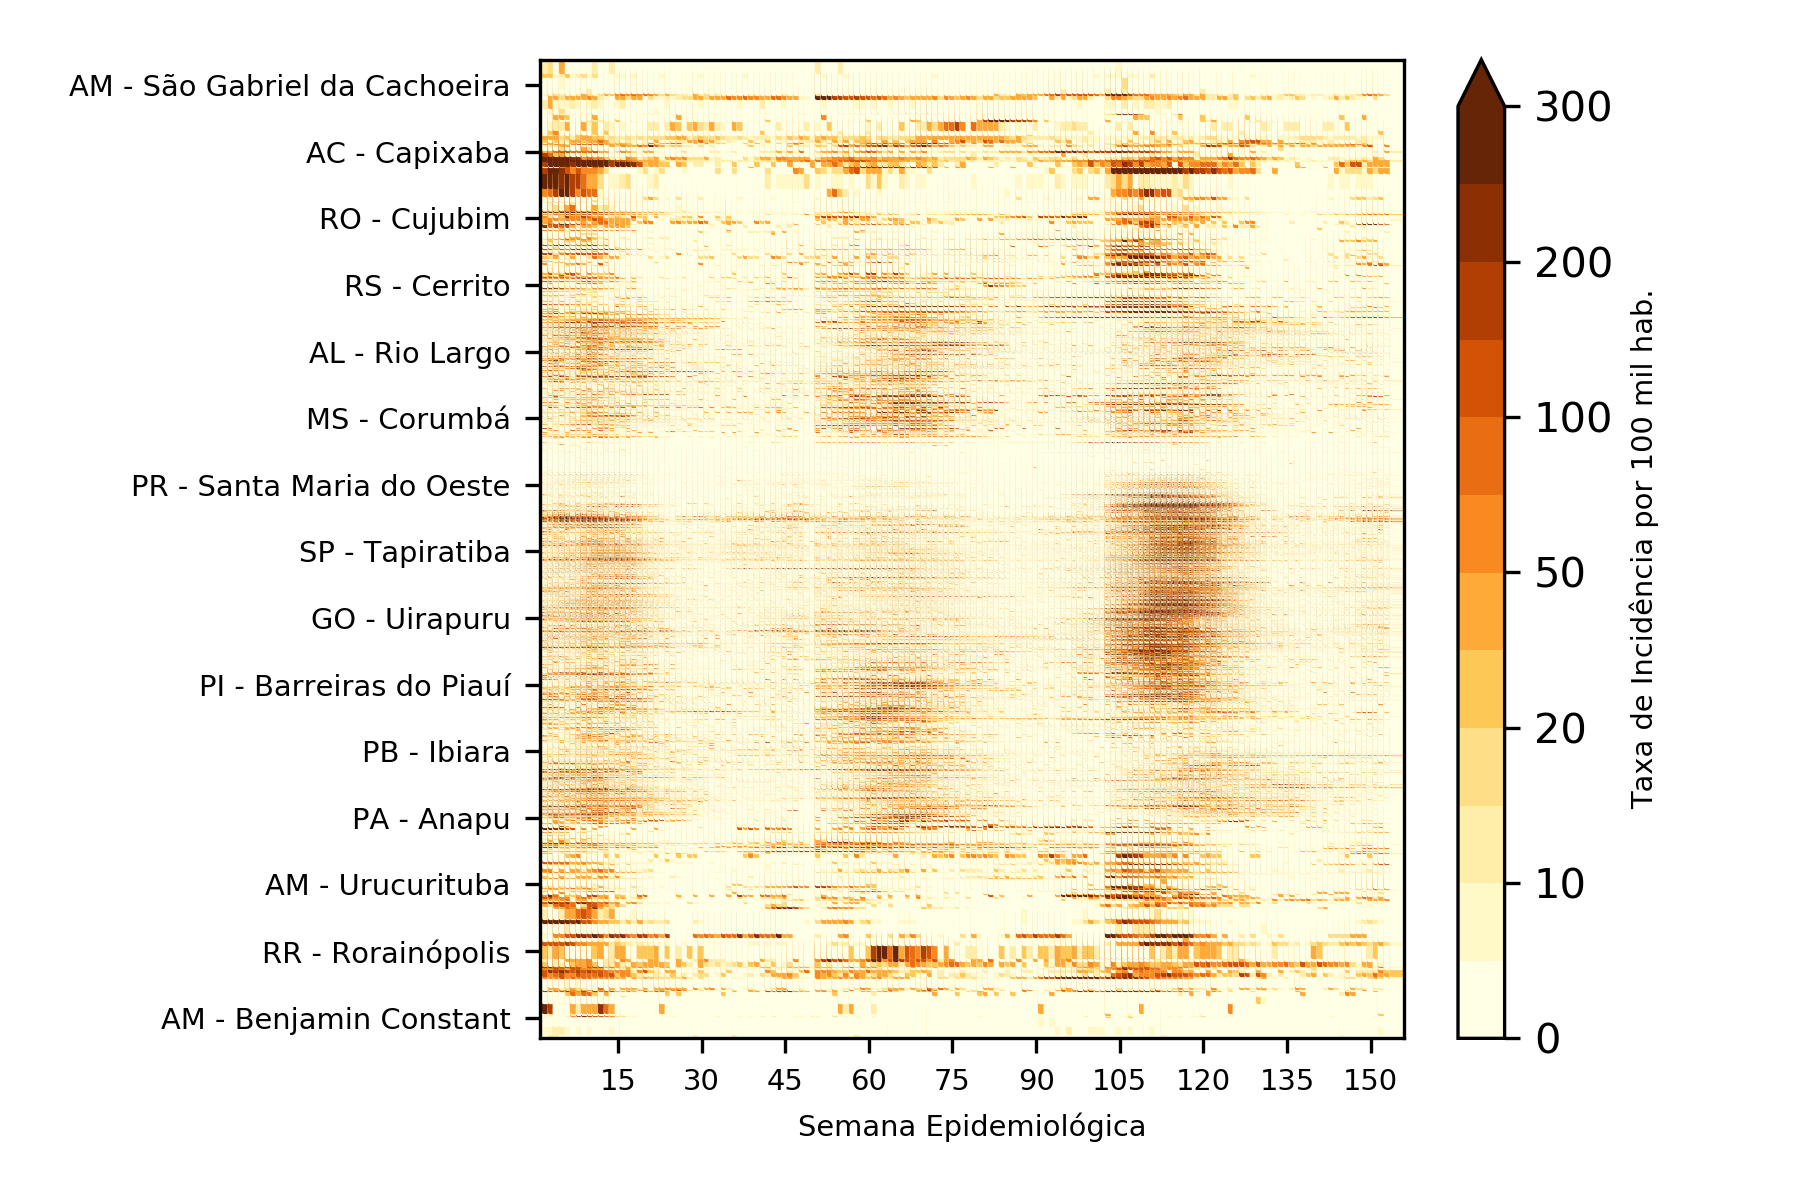
\includegraphics[width=\textwidth]{dengue-temporal_completa}}
	\caption{Representação temporal da taxa de incidência de dengue}
	\label{fig:dengue-mds}
\end{figure}

Por fim, a taxa de incidência de dengue foi representada por uma escala de cores. Essa escala de cores teve como base a quantidade de casos por 100 mil habitantes. O Ministério da Saúde define três faixas para a monitoração mensal da taxa de incidência de dengue\cite{gaussian-system-dengue}. Caso a quantidade de casos por 100 mil habitantes seja inferior a 100 (cem) é considerado que o município apresenta uma baixa taxa de incidência de dengue. A taxa entre 100 e 300, por sua vez, é classificada como incidência mediana. Por fim, caso a taxa seja superior a 300, é considerado que o município apresenta uma alta taxa de incidência da doença. Como a análise realizada nesse relatório lida com dados semanais, esse valor foi dividido por 4 (quatro). Deste modo, a escala de cores da figura \ref{fig:dengue-mds} deve ser interpretada da seguinte forma:

\begin{enumerate}[noitemsep]
	\item Incidência Baixa: até 25;
	\item Incidência Média: entre 25 e 75;
	\item Incidência Alta: maior que 75.
\end{enumerate}

A figura \ref{fig:dengue-mds} apresenta a visualização final obtida. O código-fonte \emph{python} criado para gerar a representação visual está disponível no apêndice \ref{sec:ap-codigo-mds}. A reprodução do experimento pode ser realizada fazendo o download dos dados pelo endereço: \url{https://github.com/carneirocurado/Visualizacao-Dados}.


\section{Análises}
\label{sec:analises}

Conforme pode ser observado na figura \ref{fig:dengue-mds}, a variação da taxa de incidência de dengue não é um evento isolado. Observa-se que o aumento, ou a diminuição, da taxa ocorre em vários municípios simultaneamente. Com isso, a análise da figura \ref{fig:dengue-mds} permite observar que a ocorrência de epidemias de dengue (quando a incidência é considerada alta) ocorre em ondas que afetam vários municípios simultaneamente.

Além disso, é possível observar que o nível endêmico\footnote{Chama-se de nível endêmico aquele considerado normal para a região.} de dengue varia de município para município. Deste modo, existem municípios que apresentam, ao longo de todo o período analisado, uma taxa mais alta de incidência de dengue. Entretanto, a figura \ref{fig:dengue-mds} deixa evidente que os surtos da doença ocorrem de forma simultânea em todos os municípios, sugerindo que algum fator externo influencie a ocorrência desses surtos com alguma periodicidade. Como a transmissão do vírus da dengue é muito influenciada pelo clima\cite{effect-climate-dengue}, uma possibilidade é de que as ondas de surtos da doença tenham origem na variação do clima local.

\begin{figure}[h]
	\centering
		\makebox[\textwidth]{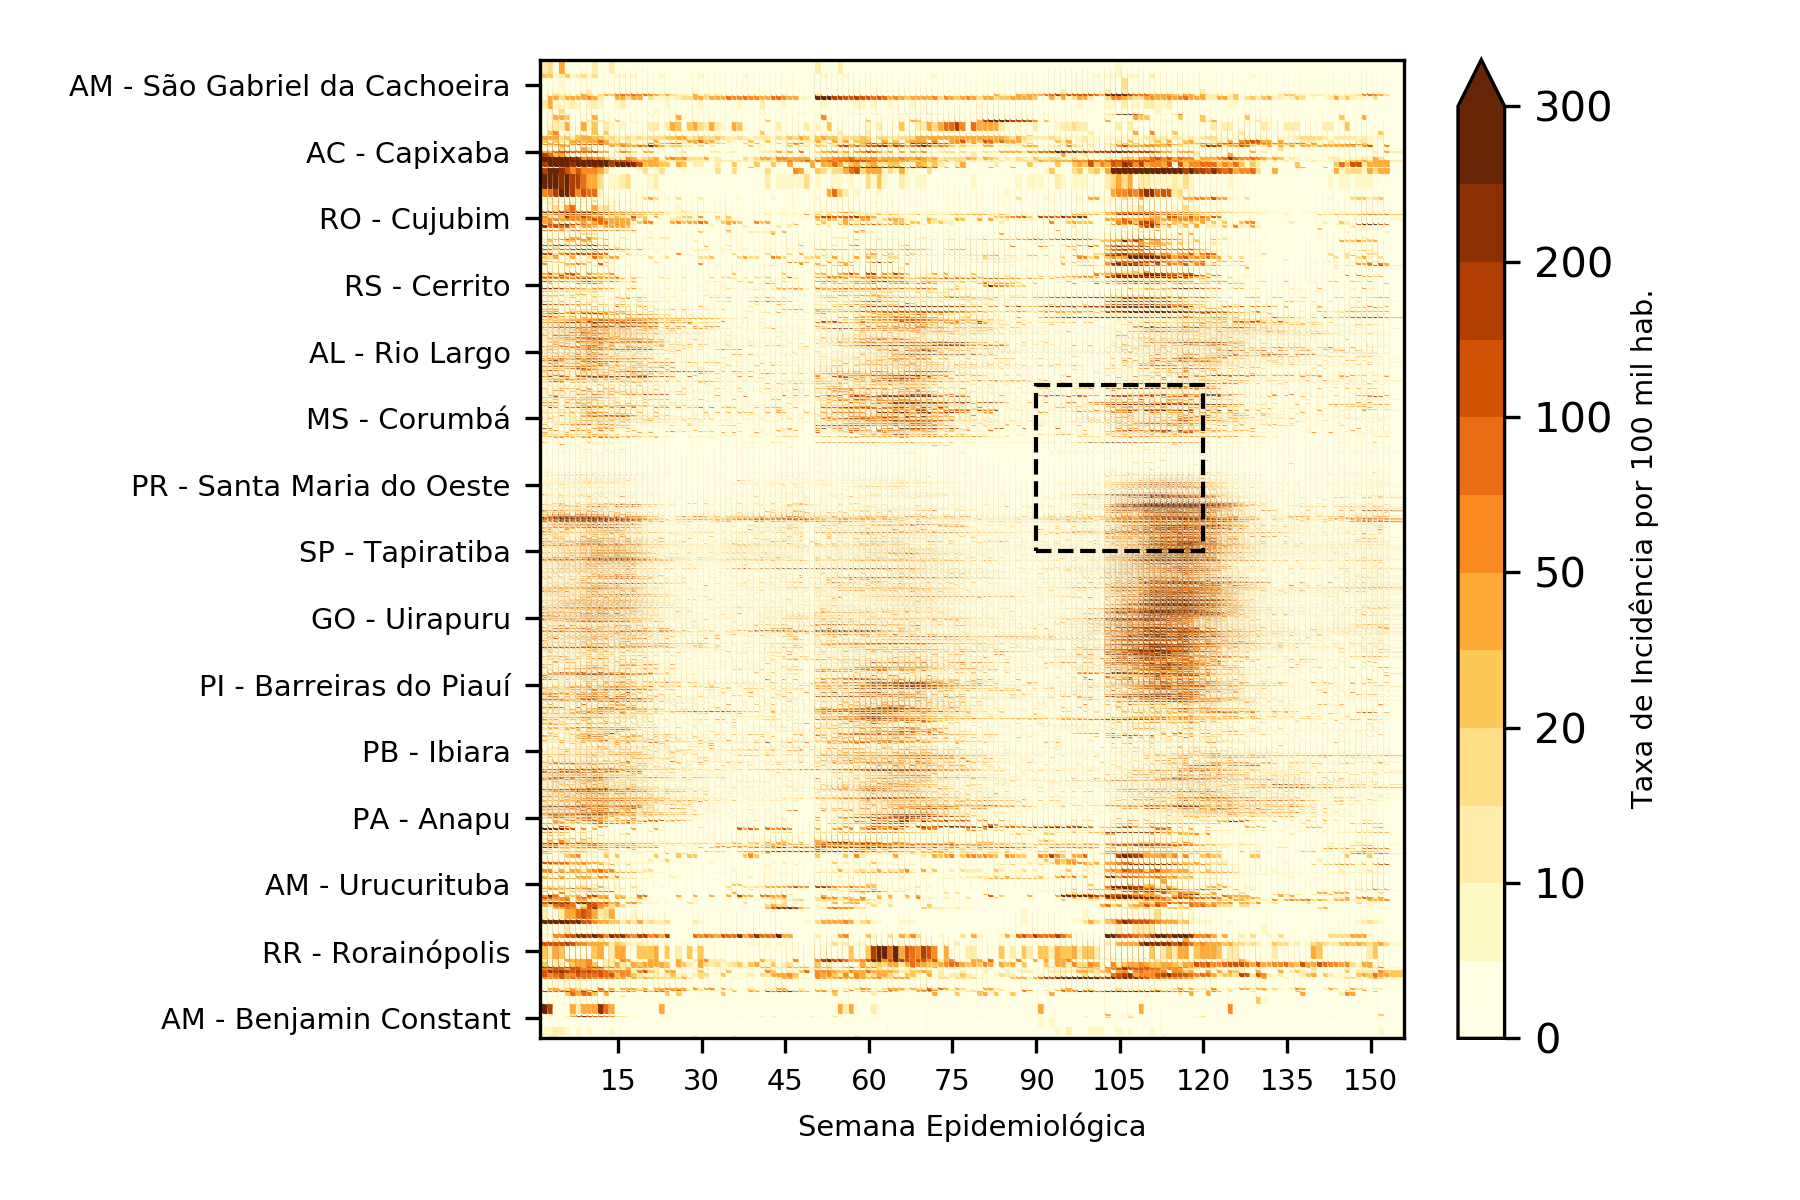
\includegraphics[width=\textwidth]{dengue-temporal_completa-destaques}}
	\caption{Representação temporal da taxa de incidência de dengue, destacando região de análise}
	\label{fig:dengue-mds-destaque}
\end{figure}

Não obstante, a análise detalhada da figura \ref{fig:dengue-mds} nos permite observar a existência de uma faixa de municípios (no eixo $y$ do gráfico) que está, constantemente, com baixa taxa de incidência de dengue. A figura \ref{fig:dengue-mds-destaque} destaca, no quadrado pontilhado, uma área do gráfico original contendo esses municípios que sempre apresentam baixa taxa de incidência de dengue. Essa área destacada corresponde, justamente, a um período no qual ocorreu surto de epidemia em praticamente todos os municípios do Brasil mas, mesmo assim, esses municípios destacados não foram afetados. A figura \ref{fig:dengue-mds-zoom} apresenta um zoom da imagem pontilhada da figura \ref{fig:dengue-mds-destaque}.

\begin{figure}[h]
	\centering
		\makebox[\textwidth]{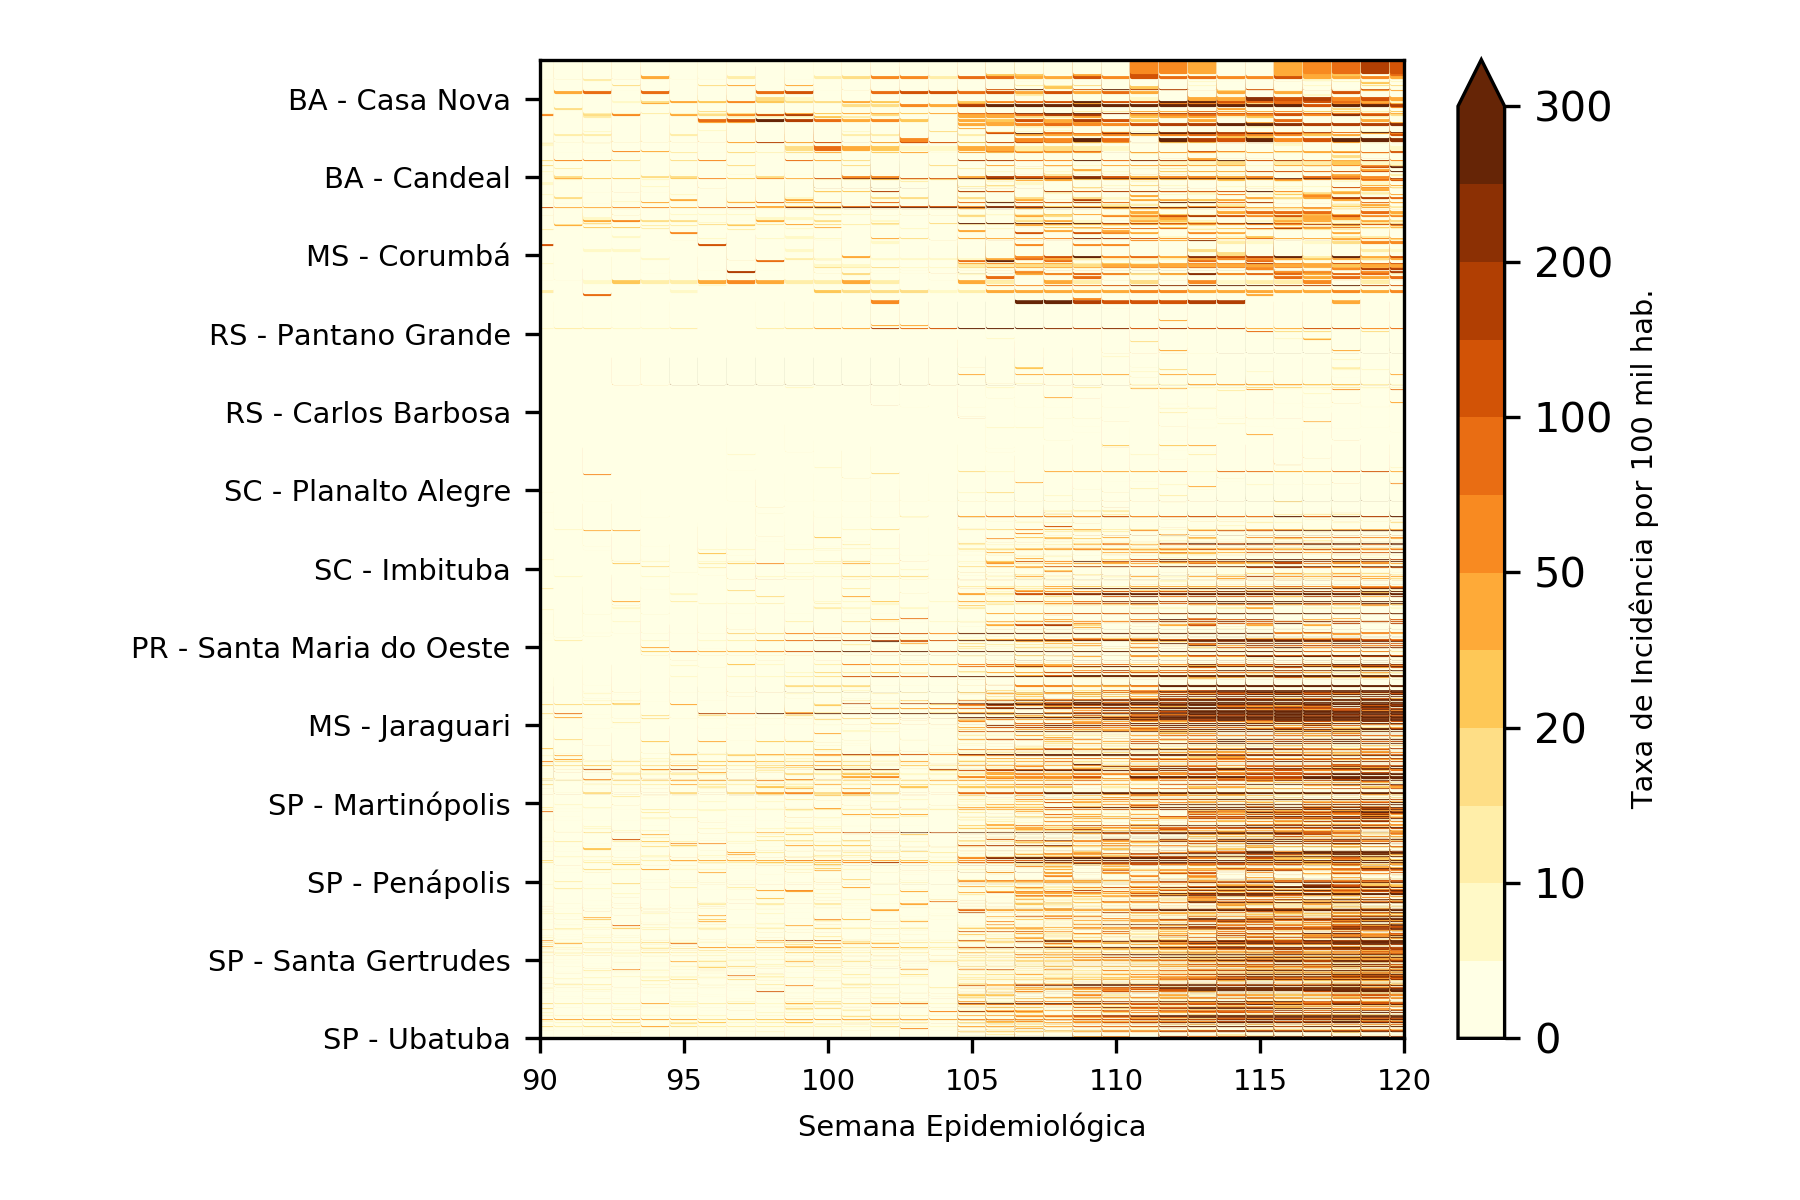
\includegraphics[width=\textwidth]{dengue-temporal_zoom}}
	\caption{Destaque da representação para municípios com baixa incidência de dengue}
	\label{fig:dengue-mds-zoom}
\end{figure}

Pode-se observar, na figura \ref{fig:dengue-mds-zoom}, que esses municípios que apresentam, constantemente, baixa taxa de incidência de dengue estão localizados no Sul do Brasil, predominantemente nos estados do Rio Grande do Sul e Santa Catarina. De acordo com o Boletim Epidemiológico do Ministério da Saúde esses são, justamente, os estados do Brasil que apresentam a menor taxa de incidência da doença\cite{ms-boletim-epidemiologico}. Cabe destacar que uma temperatura ambiente mais elevada é essencial para proliferação do mosquito da dengue\cite{effect-climate-dengue}. Deste modo, como os estados do Sul possuem um clima mais frio, esses estados são, de fato, menos propícios à proliferação do mosquito transmissor da doença.


\section{Conclusão}
\label{sec:conclusao}

A dengue é uma doença viral que apresenta a situação epidemiológica mais alarmante do mundo \cite{who-strategy-dengue-prevention}. A incidência de dengue cresceu drasticamente ao redor do mundo, afetando centenas de milhares de pessoas todo ano \cite{who-dengue-website}. Essa doença ocorre, principalmente, em áreas tropicais e subtropicais, onde as condições do meio ambiente favorecem a proliferação dos mosquitos que são os vetores de transmissão da doença \cite{ms-descricao-doenca}. Essa sensitividade às condições climáticas ocorre, principalmente, devido ao fato de os mosquitos precisarem de água parada para procriar e, também, de um ambiente quente para favorecer o desenvolvimento da larva e aumentar a velocidade de replicação do vírus \cite{effect-climate-dengue}.

A análise realizada na seção \ref{sec:analises} nos permite observar que os surtos de dengue ocorrem em ciclos. Esses ciclos podem ser claramente observados na figura \ref{fig:dengue-mds}. Provavelmente essa variação na taxa de incidência de dengue está associada à variação das condições climáticas locais, já que a proliferação do vírus está diretamente relacionada a existência de um clima quente e úmido.

Além disso, existe um grupo de municípios que aparentam ser imunes à epidemias de dengue, pois apresentam taxa de incidência dessa doença constantemente baixa. Conforme pôde ser observado nas figuras \ref{fig:dengue-mds-destaque} e \ref{fig:dengue-mds-zoom}, esses municípios estão localizados no Sul do Brasil, predominantemente nos estados de Santa Catarina e Rio Grande do Sul. Isso se deve, provavelmente, ao fato de esses municípios possuírem um clima mais frio e, portanto, menos propício à proliferação do mosquito transmissor da dengue.

A metodologia adotada na realização desse estudo teve como base a utilização da biblioteca \emph{Sklearn}\cite{sklearn-mds}. Não obstante essa biblioteca disponibilizar uma implementação do algoritmo MDS (\emph{Multidimensional Scaling}), essa implementação possui algumas limitações. A que mais impactou o trabalho foi a análise do erro gerado na redução da dimensionalidade. A redução de dimensionalidade reduz a capacidade de representação dos dados\cite{multidimensional-scaling-book}. Deste modo, existe um erro ao reduzirmos a latitude e a longitude (2 dimensões) para apenas 1 dimensão (representada no eixo $y$ dos gráficos). Esse erro é, também, chamado de \emph{stress} e o algoritmo de redução de dimensionalidade deve tentar diminuir o \emph{stress} para o menor valor possível.

Entretanto, não existe um significado claro entre o valor do \emph{stress} que a API do \emph{Sklearn} calcula e a qualidade da redução da dimensionalidade. Sabe-se que quanto mais baixo for o valor do \emph{stress}, melhor. Idealmente o \emph{stress} deveria ser zero, o que indicaria que a redução da dimensionalidade foi perfeita. A limitação encontrada na realização do presente trabalho foi, portanto, justamente em estabelecer um limite mínimo para o valor do \emph{stress} que pudesse ser considerado aceitável para a redução da dimensionalidade.

Por fim, sugere-se que trabalhos futuros explorem a visualização temporal da dengue considerando, também, fatores climáticos. Com isso, seria possível verificar se o surgimento de surtos de dengue estão, de fato, associados a variação dos fatores climáticos locais.


\backmatter

\postextual

%\pagebreak
\newpage

\bibliography{visualizacao-dados}

\apendices

%\pagebreak

\chapter{Código-fonte}
\label{sec:ap-codigo-mds}

\lstset{breaklines=true,numbers=left,extendedchars=true}

\lstset{literate=
  {á}{{\'a}}1 {é}{{\'e}}1 {í}{{\'i}}1 {ó}{{\'o}}1 {ú}{{\'u}}1
  {Á}{{\'A}}1 {É}{{\'E}}1 {Í}{{\'I}}1 {Ó}{{\'O}}1 {Ú}{{\'U}}1
  {à}{{\`a}}1 {è}{{\`e}}1 {ì}{{\`i}}1 {ò}{{\`o}}1 {ù}{{\`u}}1
  {À}{{\`A}}1 {È}{{\'E}}1 {Ì}{{\`I}}1 {Ò}{{\`O}}1 {Ù}{{\`U}}1
  {ä}{{\"a}}1 {ë}{{\"e}}1 {ï}{{\"i}}1 {ö}{{\"o}}1 {ü}{{\"u}}1
  {Ä}{{\"A}}1 {Ë}{{\"E}}1 {Ï}{{\"I}}1 {Ö}{{\"O}}1 {Ü}{{\"U}}1
  {â}{{\^a}}1 {ê}{{\^e}}1 {î}{{\^i}}1 {ô}{{\^o}}1 {û}{{\^u}}1
  {Â}{{\^A}}1 {Ê}{{\^E}}1 {Î}{{\^I}}1 {Ô}{{\^O}}1 {Û}{{\^U}}1
  {œ}{{\oe}}1 {Œ}{{\OE}}1 {æ}{{\ae}}1 {Æ}{{\AE}}1 {ß}{{\ss}}1
  {ű}{{\H{u}}}1 {Ű}{{\H{U}}}1 {ő}{{\H{o}}}1 {Ő}{{\H{O}}}1
  {ç}{{\c c}}1 {Ç}{{\c C}}1 {ø}{{\o}}1 {å}{{\r a}}1 {Å}{{\r A}}1
  {€}{{\euro}}1 {£}{{\pounds}}1 {«}{{\guillemotleft}}1
  {»}{{\guillemotright}}1 {ñ}{{\~n}}1 {Ñ}{{\~N}}1 {¿}{{?`}}1
}

\lstinputlisting[language=Python]{../codigo/dimensionalidade.py}



\end{document}
